\documentclass[a4paper,11pt]{article}
\usepackage{a4wide}
\usepackage{fullpage}
\usepackage[utf8x]{inputenc}

\usepackage[light,math]{anttor}
\usepackage[T1]{fontenc}

\usepackage[slovene]{babel}
\selectlanguage{slovene}
\usepackage[toc,page]{appendix}
\usepackage[pdftex]{graphicx} 

\usepackage{lmodern}
\usepackage{amsmath}
\usepackage{amssymb}
\usepackage{amsthm}
\usepackage{amsfonts}
\usepackage{mathtools}
\usepackage{enumitem}
\usepackage{amsfonts}
\usepackage{amsmath}
\usepackage{setspace}
\usepackage{color}
\definecolor{light-gray}{gray}{0.95}
\usepackage{listings} 
\usepackage{hyperref}
\renewcommand{\baselinestretch}{1.2} 
\renewcommand{\appendixpagename}{Priloge}

\lstset{ 
language=Matlab,
basicstyle=\footnotesize,
basicstyle=\ttfamily\footnotesize\setstretch{1},
backgroundcolor=\color{light-gray},
}

\theoremstyle{definition} 
\newtheorem*{definicija}{Definicija}
\newtheorem*{trditev}{Trditev}


\theoremstyle{plain} 
\newtheorem*{izrek}{Izrek}
\newtheorem*{posledica}{Posledica}
\newtheorem*{zgled}{Zgled}
\newtheorem{primer}{Primer}


%\DeclareMathOperator*{\inf}{inf}
%\DeclareMathOperator*{\sup}{sup}

\title{ Topološka analiza podatkov \\
\textbf{Analiza persistenčnih diagramov}
}
\author{Sara Bizjak in Žan Hafner Petrovski}
\date{12.~januar 2021}

%%%%%%%%%%%%%%%%%%%%%%%%%%%%%%%%%%%%%%%%%%%%%%%%%%%%%%%%%%%%%%%%%%%%%%%%%%%%%%%%%%%%%%%%%%%%%%%%%%%%%%%%%%%%%%%%%%%%%%%%%%%%%%%%%

\begin{document}

\maketitle

%%%%%%%%%%%%%%%%%%%%%%%%%%%%%%%%%%%%%%%%%%%%%%%%%%%%%%%%%%%%%%%%%%%%%%%%%%%%%%%%%%%%%%%%%%%%%%%%%%%%%%%%%%%%%%%%%%%%%%%%%%%%%%%%%
\begin{center}
\section*{Povzetek}
Vztrajnostni diagram Ripsovih kompleksov je prikaz razlik v zaporedju homoloških grup, ki jih porodi izbrana filtracija. 
Zanima nas stabilnost vztrajnostnih diagramov na konkretnih primerih, empirično torej raziščemo vpliv perturbacije vhodnih točk. 
Vpliv merimo z razdaljo bottleneck, katere porazdelitev primerjamo z normalno porazdelitvijo. 
Ugotovimo, da razdalje niso normalno porazdeljene. 
\end{center}

%%%%%%%%%%%%%%%%%%%%%%%%%%%%%%%%%%%%%%%%%%%%%%%%%%%%%%%%%%%%%%%%%%%%%%%%%%%%%%%%%%%%%%%%%%%%%%%%%%%%%%%%%%%%%%%%%%%%%%%%%%%%%%%%%

\section{Uvod}
\ \ \ \
V članku so predstavljena orodja in rezultati, ki smo jih dobili po testiranju implementacije filtracij 
Ripsovega kompleska in nadaljnji analizi stabilnosti vztrajnostnih diagramov na izbranih množicah točk.
Natančneje, topološke značilnosti Ripsovih kompleksov v izbrani filtraciji zakodiramo v vztrajnostni diagram in preučujemo stabilnost tega kodiranja.
Zanimalo nas bo torej, če se z majhno perturbacijo izbranih točk tudi vztrajnostni diagram ustrezno malo spremeni.
Konstruirane vztrajnostne diagrame med sabo primerjamo tako, da izračunamo razdalje med originalnim diagramom in tistimi, ki jih dobimo s perturbiranjem začetnih točk. 
Na teh meritvah razdalj izvedemo osnovno statistiko in dobljeno porazdelitev primerjamo z normalno.

Prvi del članka opiše teoretično ozadje problema. Najprej se seznanimo s prvotnim problemom. 
Opišemo pojme, ki jih je potrebno razumeti pred samo implementacijo in si ogledamo orodja in postopke, s katerimi smo rešili dani problem. 
V drugem delu predstavimo rezultate izvedene analize.

%%%%%%%%%%%%%%%%%%%%%%%%%%%%%%%%%%%%%%%%%%%%%%%%%%%%%%%%%%%%%%%%%%%%%%%%%%%%%%%%%%%%%%%%%%%%%%%%%%%%%%%%%%%%%%%%%%%%%%%%%%%%%%%%%

\section{Metode}

%%%%%%%%%%%%%%%%%%%%%%%%%%%%%%%%%%%%%%%%%%%%%%%%%%%%%%

\subsection{Teoretično ozadje}

\ \ \ \
To podpoglavje je namenjeno uvedbi pojmov in postopkov, ki so potrebni za izvedbo implementacije in pripadajoče analize.

\begin{definicija}
    \textit{Ripsov kompleks} za množico točk $S$ in radij $r$, ki ga označimo z Rips$(S, r)$, je abstraktni simplicialni kompleks, za katerega velja:
    \begin{itemize}
        \item množica oglišč je enaka množici $S$,
        \item podmnožica $\sigma \subseteq S$ je simpleks natanko tedaj, ko je premer $\sigma$ največ $r$.
    \end{itemize}
\end{definicija}

Zgornja definicija nam pove, da je $\sigma \subseteq S$ simpleks v Ripsovem kompleksu Rips$(S, r)$ natanko takrat, 
kadar je presek dveh zaprtih krogel s premerom $r$ v katerih koli dveh točkah iz $\sigma$ neprazen.

\begin{definicija}
    \textit{Filtracija} za kompleks $K$ je definirana kot naraščajoče zaporedje kompleksov
    $$
    \emptyset \neq K_0 \leq K_1 \leq \ldots \leq K_n = K.
    $$
    Filtraciji ustreza tudi zaporedje $p$-te homološke grupe, kar lahko zapišemo
    $$
    \emptyset \neq H_p(K_0) \leq H_p(K_1) \leq \ldots \leq H_p(K_n) = H_p(K).
    $$
\end{definicija}
\noindent
Vemo, da vsako homološko grupo generirajo t.~i. generatorji grup. Rečemo, da se generator $\gamma$ v $H_p(K_i)$ za $i = 0, \ldots, r$
\begin{itemize}
    \item \textit{rodi} ob času (radiju) $i$, če $\gamma \notin H_p(K_{i-1})$ in $\gamma \in H_p(K_i)$,
    \item \textit{umre} ob času (radiju) $j$, če $\gamma \in H_p(K_{j - 1})$ in ni neodvisen generator v $H_p(K_j)$.
\end{itemize}

\begin{definicija}
    \textit{Vztrajnostni diagram} je prikaz vseh točk $(i, j)$ v ravnini $\mathbb{R}^2$, ki jih dodelimo vsakemu generatorju $\gamma \in H_p(K_l)$ za nek $l$. Pri tem $i$ označuje rojstvo, $j$ pa smrt generatorjev.
\end{definicija}
\noindent
Z besedami, na vztrajnostnem diagramu označimo stanje, ko se dva generatorja homoloških grup združita. 
Prikaz pomeni, da prejšnji generator ob tem času (oz. ob tem radiju) umre, novi združeni generator pa se rodi. 
\\

Da bi analizirali stabilnost vztrajnostnih diagramov, poskušamo odgovoriti na vprašanje, kako majhne spremembe začetnih podatkov vplivajo na diagram.
Zanimalo nas bo torej, če se z majhno perturbacijo začetnih točk tudi vztrajnostni diagram ustrezno malo spremeni.
Stabilnost lahko seveda poskusimo ugotoviti z opazovanjem vztrajnostnih diagramov, vendar si želimo formalnejšega in bolj objektivnega pristopa, 
zato vpeljemo še pojem razdalje bottleneck, ki nam poda razdaljo med dvema diagramoma.

\begin{definicija}
    Razdalja bottleneck med vztrajnostnima diagramoma $X$ in $Y$ je definirana kot
    \[
    W_{\infty}(X, Y) = \inf_{\varphi: X \rightarrow Y} \left( \sup_{x \in X} || x - \varphi(x) ||_{\infty} \right).
    \]
\end{definicija}
\noindent
Da bi empirično pokazali stabilnost vztrajnostnih diagramov, moramo zadostiti naslednji trditvi.

\begin{trditev}
    Naj bo $S = \{v_1, v_2, \ldots, v_n \}$ množica točk, ki ji priredimo $\epsilon$-perturbacijo $S' = \{v_1', v_2', \ldots, v_n' \}$, tako da velja
    $$
    d(v_i, v_i') \leq \epsilon, \ \ \forall i \in \{1, 2, \ldots, n \}.
    $$
    Tedaj je razdalja bottleneck med vztrajnostnima diagramoma pripadajočih Ripsovih kompleksov največ $2 \epsilon$:
    $$
    d_b(D(S), D(S')) \leq 2 \epsilon.
    $$
\end{trditev}

%%%%%%%%%%%%%%%%%%%%%%%%%%%%%%%%%%%%%%%%%%%%%%%%%%%%%%

\subsection{Opis problema in implementacija}
\ \ \ \
V problemu, ki ga rešujemo, je filtracija porojena z naraščanjem parametra $r$ za Ripsov kompeks, ki ji ustreza tudi zaporedje homoloških grup.
Če si predstavljamo gradnjo Ripsa tako, da okoli točk konstruiramo zaprte krogle in opazujemo njihove preseke, potem lahko rečemo, da skozi to filtracijo večamo polmer oz. premer teh krogel.
Zanima nas, kako se oblika Ripsovega kompleksa razvija skozi filtracijo, tj. kako se spreminja z večanjem parametra $r$. 
Vse te razlike v zaporedju homoloških grup, ki jih porodi filtracija, so zakodirane in predstavljene z vztrajnostnim diagramom. 
Cilj je predstaviti stabilnost vztrajnostnih diagramov Vietoris-Ripsovih kompleksov na izbranih množicah točk.
Najprej je potrebno narediti particijo

\begin{equation}\label{eq:r}
     0 = r_0 < r_1 < \ldots < r_{10} = R,
\end{equation}
\noindent
ki interval $[0, R]$, kjer je $R$ premer množice, razdeli na 10 enakih delov. 
Za vse izračunane $r_i$ zgradimo Ripsove komplekse, kar nam da filtracijo 

\begin{equation}\label{eq:filtr}
    Rips(S, r_0) \leq Rips(S, r_1) \leq \ldots \leq Rips(S, r_{10}).
\end{equation}
\noindent
V podani filtraciji je kompleks $Rips(S, r_0)$ enak množici točk $S$, v Rips$(S,r_{10})$ pa je simpleks kar vsaka podmnožica množice $S$, saj je $r_{10}$ definiran kot premer $S$.
\\
Opisan postopek še 100-krat ponovimo na točkah, ki jim dodamo šum velikosti $\epsilon < \frac{R}{100}$. Dodajanje šuma oz. perturbacija točk je prikazana na sliki \ref{slika:orig_noise}.

\begin{figure}[ht!]
    \centering
    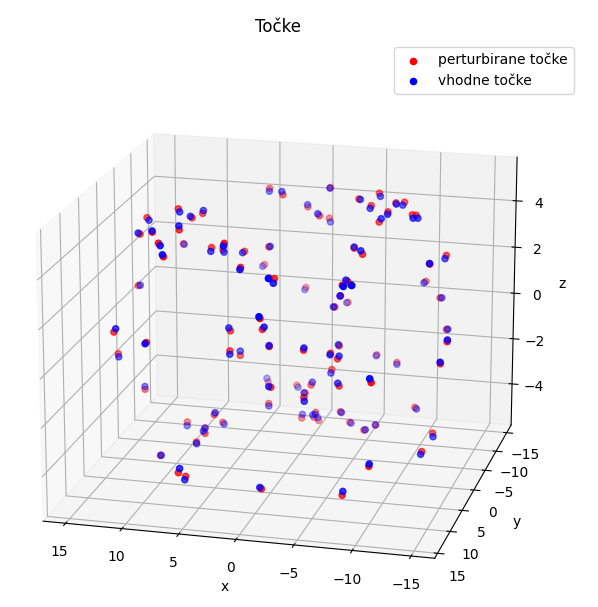
\includegraphics[width=80mm]{../slike/orig_noise3d.png}
    \caption{Prikaz ene izmed podanih množic točk in ene izmed njenih perturbacij.}
    \label{slika:orig_noise}
\end{figure}
\noindent
Za vse filtracije Ripsovih kompleksov (zgrajenih na prvotnih in perturbiranih točkah) zgradimo vztrajnostne diagrame v dimenzijah 0, 1 in 2 ter jih primerjamo.
Gradnja vztrajnostnega diagrama za izvorno množico točk je prikazana na sliki \ref{slika:tocke_diag}.

\begin{figure}[ht!]
    \centering
    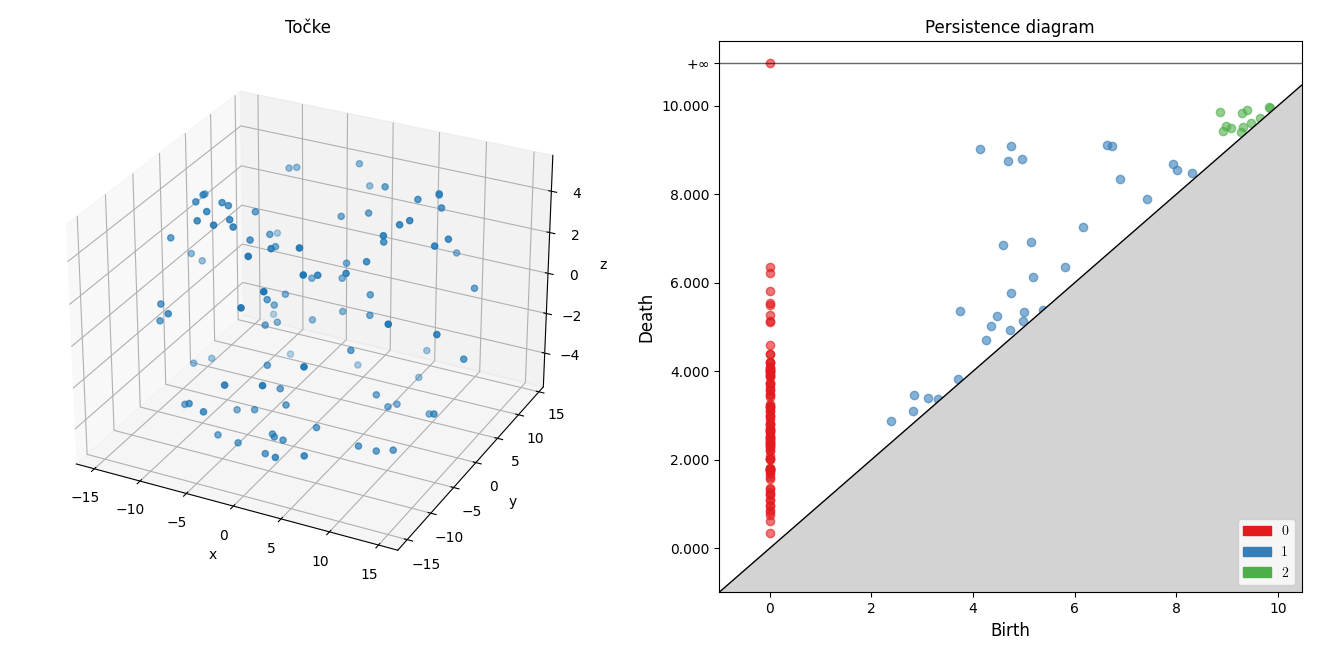
\includegraphics[width=150mm]{../slike/tocke3d_02_diagram.png}
    \caption{Prikaz izvornih točk in vztrajnostnega diagrama pripadajoče Ripsove filtracije.}
    \label{slika:tocke_diag}
\end{figure}
\noindent
Za vsak vztrajnostni diagram, zgrajen na perturbiranih točkah, izračunamo razdaljo bottleneck od prvotnega vztrajnostnega diagrama za vsako dimenzijo posebej.
Na sliki \ref{slika:10particij} so prikazani histogrami vseh razdalj bottleneck za dimenzije 0, 1 in 2, ki jih dobimo z zgoraj opisanim postopkom.

\begin{figure}[ht!]
    \centering
    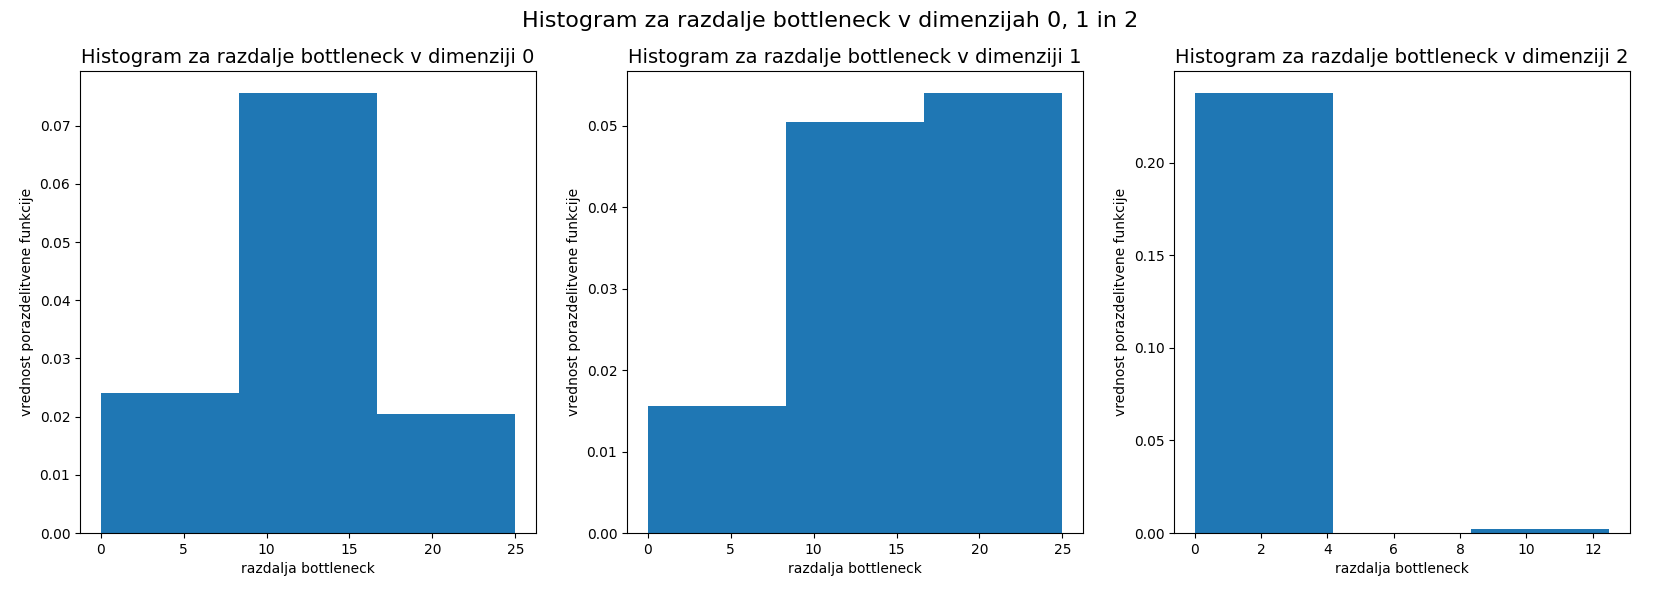
\includegraphics[width=165mm]{../slike/bottleneck_pers02_100samples_10partpoints_dim012.png}
    \caption{Razdalje bottleneck vztrajnostnih diagramov v dimenziji 0, 1 in 2 za množico s 100 točkami pri filtraciji, kot je zapisano v \ref{eq:filtr}.}
    \label{slika:10particij}
\end{figure}

Ker je na rezultatih, pridobljenih na podlagi particije na 10 delov, težko narediti zaključke, se odločimo raje za finejšo particijo. 
Naredimo najfinejšo možno filtracijo za Ripsove komplekse, kot jo ponuja knjižnica \texttt{gudhi}. 
Za še boljše in bolj relevantne rezultate -- namesto 100 -- zgradimo 1000 množic s perturbiranimi točkami.
Na dobljenih rezultatih izvedemo nekaj osnovne statistike in jih primerjamo z normalno porazdelitvijo.
\\

Za implementacijo funkcij in analizo je bil uporabljen programski jezik \texttt{Python}.
Za gradnjo Ripsovih kompleksov v filtraciji in vztrajnostnih diagramov je bila v največji meri uporabljena že vgrajena knjižnica \texttt{gudhi}, 
za test normalne porazdelitve pa smo uporabili \textit{Spahiro-Wilkov test}, ki je vgrajen v knjižnici \texttt{scipy.stats}.
Analiza in testi so dostopni v priloženi datoteki \texttt{analysis.py}, funkcije, ki smo jih uporabljali, pa v datoteki \texttt{helper\_functions.py}.

%%%%%%%%%%%%%%%%%%%%%%%%%%%%%%%%%%%%%%%%%%%%%%%%%%%%%%%%%%%%%%%%%%%%%%%%%%%%%%%%%%%%%%%%%%%%%%%%%%%%%%%%%%%%%%%%%%%%%%%%%%%%%%%%%

\section{Rezultati}

\ \ \ \ 
V tem poglavju so prikazani rezultati, dobljeni z najfinejšo možno filtracijo, in statistika, 
narejena na 1000 ponovitvah s perturbiranimi točkami iz datotek \texttt{persistence01\_100.out} in \texttt{persistence02\_100.out}.
\\

Na spodnjih slikah so prikazani histrogrami vseh dobljenih razdalj bottleneck med izvornim in vsemi vztrajnostnimi diagrami, dobljenimi na podlagi perturbiranih točk, za dimenzije 0, 1 in 2.
Na vsakem histogramu je z rdečo barvo označeno povprečje razdalj bottleneck in z zeleno barvo $\epsilon$, ki predstavlja šum, s katerim smo zmotili izvorne točke.
Z oranžno barvo je označena normalna porazdelitev za ustrezne parametre, torej za izračunano povprečje razdalj in varianco za posamezni primer.
\\

\begin{figure}[ht!]
    \begin{minipage}{0.5\textwidth}
        \centering
        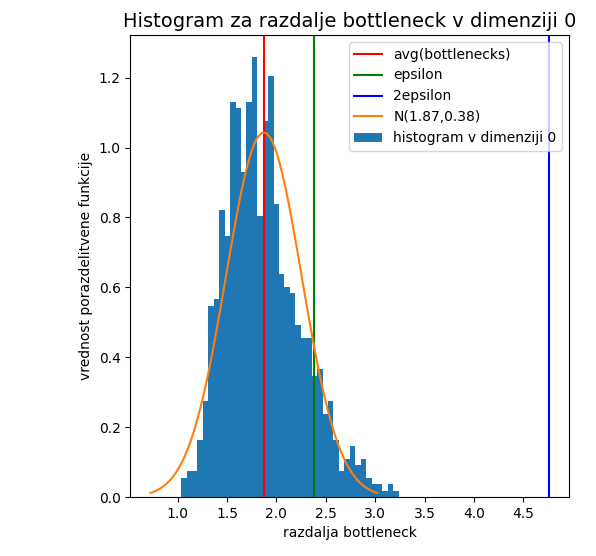
\includegraphics[width=82mm]{../slike/bottleneck_1000_dim0.png}
        \label{slika:hist1_0}
    \end{minipage}\hfill
    \begin{minipage}{0.5\textwidth}
        \centering
        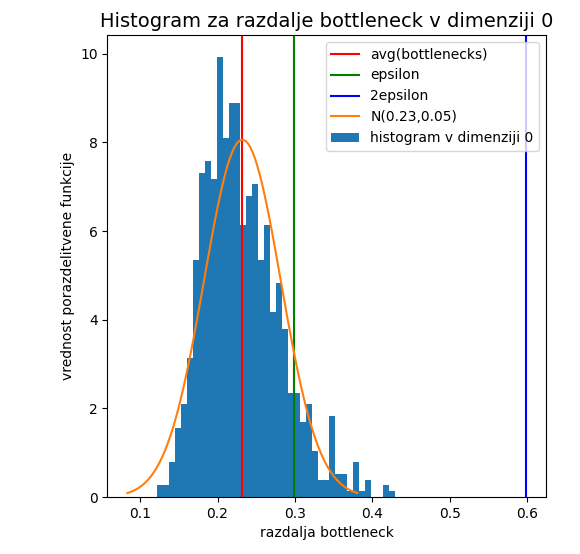
\includegraphics[width=79mm]{../slike/bottleneck2_1000_dim0.png}
        \label{slika:hist2_0}
    \end{minipage}\hfill
    \caption{Primerjava razdalje bottleneck vztrajnostnih diagramov v dimenziji 0 z normalno porazdelitvijo za dve različni izvorni množici s 100 točkami.}
\end{figure}

\begin{figure}[ht!]
    \begin{minipage}{0.5\textwidth}
        \centering
        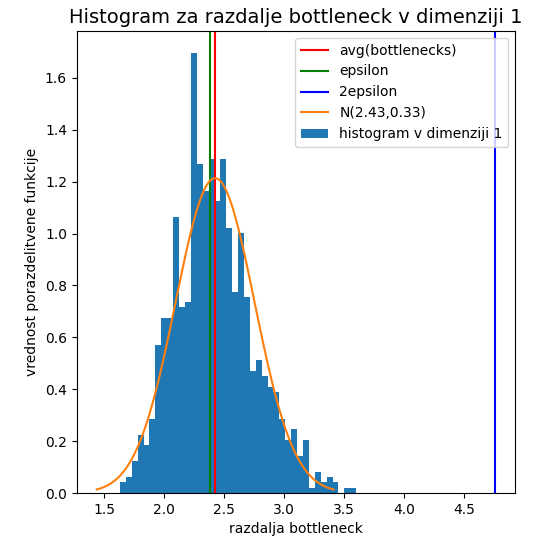
\includegraphics[width=82mm]{../slike/bottleneck_1000_dim1.png}
        \label{slika:hist1_1}
    \end{minipage}\hfill
    \begin{minipage}{0.5\textwidth}
        \centering
        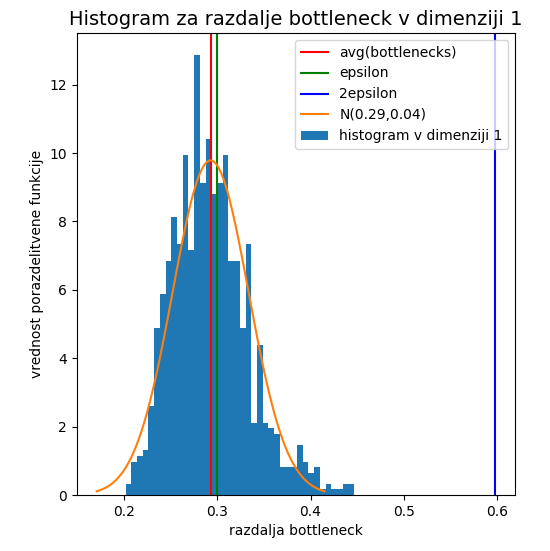
\includegraphics[width=82mm]{../slike/bottleneck2_1000_dim1.png}
        \label{slika:hist2_1}
    \end{minipage}\hfill
    \caption{Primerjava razdalje bottleneck vztrajnostnih diagramov v dimenziji 1 z normalno porazdelitvijo za dve različni izvorni množici s 100 točkami.}
\end{figure}

\begin{figure}[ht!]
    \begin{minipage}{0.5\textwidth}
        \centering
        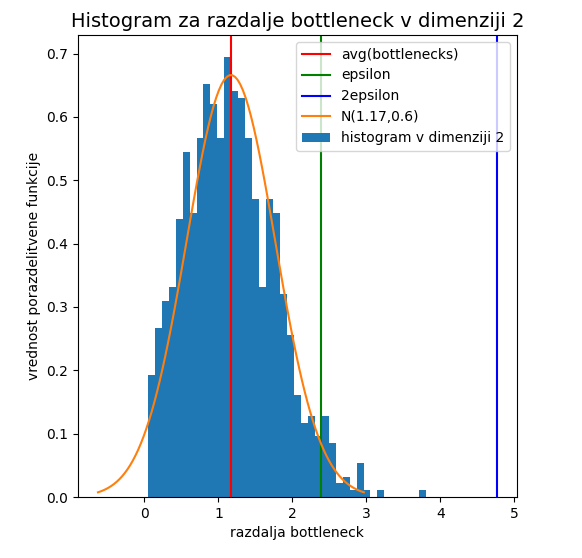
\includegraphics[width=85mm]{../slike/bottleneck_1000_dim2.png}
        \label{slika:hist1_2}
    \end{minipage}\hfill
    \begin{minipage}{0.5\textwidth}
        \centering
        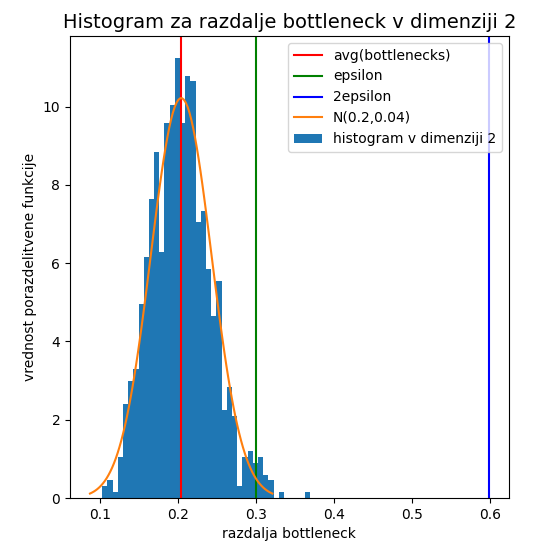
\includegraphics[width=81mm]{../slike/bottleneck2_1000_dim2.png}
        \label{slika:hist2_2}
    \end{minipage}\hfill
    \caption{Primerjava razdalje bottleneck vztrajnostnih diagramov v dimenziji 2 z normalno porazdelitvijo za dve različni izvorni množici s 100 točkami.}
\end{figure}

\newpage
Če je pri 100 ponovitvah na oko še izgledalo, da bi bila porazdelitev morda lahko normalna, pa se na teh histogramih za 1000 ponovitev perturbiranja točk hitro vidi, da je histogram preveč nagnjen v levo, da bi bil lahko normalno porazdeljen.
Da bi opazovanja tudi računsko potrdili, smo izvedli Shapiro-Wilkov test normalnosti, ki potrdi, da porazdelitev v nobenem primeru dimenzije ni normalna. 
V vseh dimenzijah je bila $p-$vrednost manjša od števila $10^{-5}$, kar vidimo tudi v tabeli \ref{tabela:p}. Ker so $p-$vrednosti manjše od $0.05$, zavrnemo hipotezo o normalni porazdelitvi.

\begin{table}[ht!]
    \centering
    \begin{tabular}{|l|c|c|}
    \hline
    dimenzija \textbackslash \ datoteka & \texttt{persistence01\_100} & \texttt{persistence02\_100} \\ \hline
    0                                 & 3.645e-13          & 9.648e-15          \\ \hline
    1                                 & 9.993e-08          & 2.873e-12          \\ \hline
    2                                 & 7.845e-10          & 3.802e-06          \\ \hline
    \end{tabular}
    \caption{Izračunane $p-$vrednosti s Shapiro-Wilkovin testom.}
    \label{tabela:p}
\end{table}
\noindent
Zanimivo je še opaziti, da se povprečna bottleneck razdalja giblje pod ali pa okoli vrednosti $\epsilon$.

Nadalje opazimo tudi, da so vse razdalje bottleneck manjše od $2 \epsilon$, kar empirično potrdi že zapisana trditev o stabilnosti vztrajnostnih diagramov za Ripsove komplekse.
Tudi subjektivna ocena na podlagi vztrajnostnega diagrama na izvornih in perturbiranih točkah sledi tej opazki, saj se vztrajnostna diagrama tudi na oko ustrezno malo razlikujeta.

\begin{figure}[ht!]
    \centering
    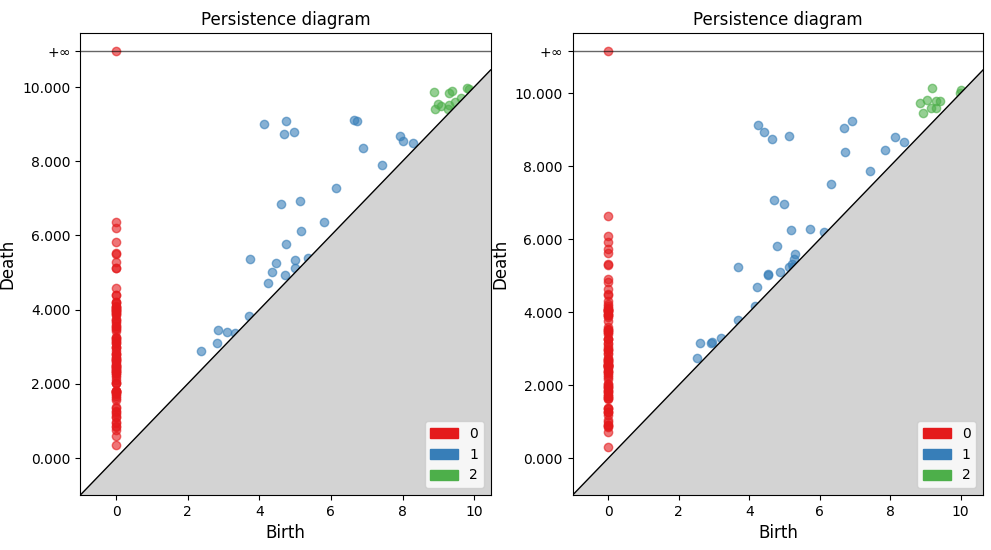
\includegraphics[width=150mm]{../slike/primerjava_diagramov.png}
    \caption{Levo je prikazan vztrajnostni diagram za izvorne točke, desno pa za perturbirane.}
    \label{slika:primerjava}
\end{figure}

%%%%%%%%%%%%%%%%%%%%%%%%%%%%%%%%%%%%%%%%%%%%%%%%%%%%%%%%%%%%%%%%%%%%%%%%%%%%%%%%%%%%%%%%%%%%%%%%%%%%%%%%%%%%%%%%%%%%%%%%%%%%%%%%%

\section{Zaključek}
\ \ \ \ 
Odločitev o finejši filtraciji in izračunu 1000 vrednosti razdalje bottleneck namesto 100 se je izkazala za dobro, saj smo histograme lahko tako bolj kredibilno primerjali z normalno poradelitvijo.
Videli smo, da porazdelitve razdalj bottleneck niso normalne, empirično pa smo potrdili tudi trditev o stabilnosti vztrajnostnih diagramov Ripsovih kompleksov.


%%%%%%%%%%%%%%%%%%%%%%%%%%%%%%%%%%%%%%%%%%%%%%%%%%%%%%%%%%%%%%%%%%%%%%%%%%%%%%%%%%%%%%%%%%%%%%%%%%%%%%%%%%%%%%%%%%%%%%%%%%%%%%%%%

\begin{thebibliography}{99}

    \bibitem{bib:tap}
    Zapiski po predavanjih profesorja Ž.~Virka in profesorice N.~Mramor Kosta pri predmetu \emph{Topološka analiza podatkov}, šolsko leto 2020/2021.
    
\end{thebibliography}


\end{document}